\documentclass[12pt,a4paper,draft]{article}

\usepackage[utf8]{inputenc}
\usepackage[spanish]{babel}
\usepackage[numbers,sort&compress]{natbib}
\usepackage{amsmath}
\usepackage{amsfonts}
\usepackage{amssymb}
\usepackage{graphicx}
\usepackage[left=2cm,right=2cm,top=2cm,bottom=2cm]{geometry}

\author{Cynthia Ivanna Cruz Quiñones\\
Matricula: 1854499\\
Grupo: 002}
\title{Matemáticas Computacionales\\
Practica 1}
\date{A 16 de Febrero del 2021}


\begin{document}
\maketitle

\newpage
\tableofcontents

\newpage

\section{Introdcción}
En esta primera práctica se hará una de las cosas básicas al momento de aprende R. Se
repasaran las curvas en $\mathbb{R}^2$ vistas en primer semestre en la materia de Geometría Analítica. [1].
Se graficarán curvas como la recta, parábola, circunferencia, elipse e hipérbola.
\section{Curvas de $\mathbb{R}^2$} \label{sec:curvas}

\subsection{Línea recta} \label{subsec:linearecta}
\textbf{Definición}
Llamamos línea recta al lugar geométrico de los puntos tales que tomados dos puntos diferentes cualesquiera $P_{1}(x_{1}, y_{1})$ y $P_{2}(x_{2}, y_{2})$ del lugar, el valor de la pendiente $m$ calculado por medio de la fórmula 

$$ m = \frac{y_{1} - y_{2}}{x_{1} - x_{2}}$$ 

,tal que  ${x_{1}\neq x_{2}}$, resulta siempre constante. 

La formula general es
$$Ax + By + C = 0$$

La ecuación pendiente-ordenada al origen
$$y = mx + b$$

\subsubsection{Ejemplos: Linea Recta}

\begin{figure}
\centering 
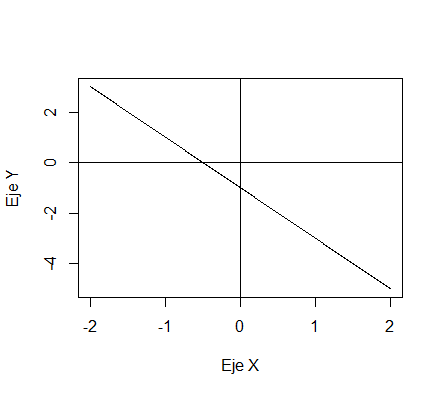
\includegraphics[scale=0.5]{Recta1}
\caption{Ejemplo 1 de linea recta}
\end{figure}



\subsection{Parábola} \label{subsec:parabola}
\textbf{Definición} Una parábola es el lugar geométrico de un punto que se mueve en un plano de tal manera que su distancia de una recta fija, situada en el plano , en siempre igual a la distancia de un punto fijo del plano y que no pertenece a la recta.
El punto fijo se llama $foco$ y la recta fija $directriz$ de la parábola.

La ecuacion de una parábola de vértice en el origen y el eje X, es 
$$y^2 = 4px$$
en donde el foco es el punto $(p,0)$ y la ecuación de la directriz es $x = -p$. Si $p > 0$, la parábola se abre hacia la derecha; si $p < 0$, la parabola se abre hacia la izquierda.

Si el eje de una parábola coincide con el eje Y, el vértice está en el origen, su ecuaciñon es 
$$x^2 = 4py$$
en donde el foco es el punto $(0,p)$, y la ecuación de la directriz es $y = -p$. Si $p > 0$, la parábola se abre hacia arriba; si $p < 0$, la parabola se abre hacia la abajo.

En cada caso, la longitud del lado recto está dada por el valor absoluto de 4p, que es el coeficiente del término de primer grado.

La ecuacion de una parábola de vértice $(h,k)$ y eje paralelo al eje X, es de la forma
$$(y - k)^2 = 4p(x - h)$$
Si $p > 0$, la parábola se abre hacia la derecha; si $p < 0$, la parábola se abre hacia la izquierda.
En cambio, si el vértice es el punto $(h,k)$ y el eje de la parábola es paralelo al eje Y, su ecuación es de la forma 
$$(x - h)^2 = 4p(y - k)$$
Si $p > 0$, la parábola se abre hacia arriba; si $p < 0$, la parábola se abre hacia abajo.

\subsubsection{Ejemplos: Parábola}

\subsection{Circunferencia} \label{subsec:circunferencia}
\textbf{Definición} La circunferencia es el lugar geométrico de un punto que se mueve en el plano de tal manera que se conserva siempre a una constante llamada $radio$

La $circunferencia$ cuyo centro es el punto (h,k) y $cuyo radio$ es la constante $r$, tiene por ecuación

$${(x - h)^2 + (y - k)^2 = r^2}$$

\subsubsection{Ejemplos: Circunferencia}

\subsection{Elipse}
\textbf{Definición} Una $elipse$ es el lugar geométrico de un punto que se mueve en un plano de tal manera que la suma de sus distancias a dos puntos fijos de este plano es siempre igual a una constante, mayor que la distancia entre los dos puntos.
\\Los dos puntos fijos se llaman $focos$ de la elipse. 


La ecuación de la elipse de centro en el origen, eje focal coincidente con el $eje X$, y focos los puntos $(c,0)$ y $(-c,0)$, es
$$ {\frac{x^2}{a^2} + \frac{y^2}{b^2} = 1} $$

Si el eje focal coincide con el $eje Y$, de manera que las coordenadas de los focos $(0,c$) y $(0,-c)$, entonces la ecuación es 
$$ {\frac{y^2}{a^2} + \frac{x^2}{b^2} = 1} $$

Ecuacion de la hipérbola con eje transversal $horizontal$
$$ {\frac{(x - h)^2}{a^2} + \frac{(y - k)^2}{b^2} = 1} $$

Ecuacion de la hipérbola con eje transversal $vertical$
$$ {\frac{(x - k)^2}{a^2} + \frac{(y - h)^2}{b^2} = 1} $$

Para cada elipse $a$ es la longitud del semejante mayor, $b$ la del semejante menor, $c$ la distancia del centro a cada foco, y $a$, $b$, $c$ estan ligadas por la relacion $a^2 = b^2 + c^2$.
\\También, para cada elipse, la longitud de cada uno de sus lados rectos es $\frac{2b^2}{a}$, y la excentridad $e$ está dada por la relación.

$$e = \frac{c}{a} = \frac{\sqrt{a^2 - b^2}}{a} < 1$$

\subsubsection{Ejemplos: Elipse}

\subsection{Hipérbola}
\textbf{Definición} La hipérbola es el lugar geométrico de un punto que se mueve en un plano de tal manera que el valor absoluto de la diferencia de sis distancias a dos puntos fijos del plano, llamados $focos$, es siempre iguala una cantidad constante, positiva y menor que la distancia entre los focos.

La ecuación de la hipérbola de centro en el origen, eje focal coincidente con el $eje X$, y focos los puntos $(c,0)$ y $(-c,0)$, es
$$ {\frac{x^2}{a^2} - \frac{y^2}{b^2} = 1} $$

Si el eje focal coincide con el $eje Y$, de manera que las coordenadas de los focos $(0,c$) y $(0,-c)$, entonces la ecuación es 
$$ {\frac{y^2}{a^2} - \frac{x^2}{b^2} = 1} $$

Ecuacion de la hipérbola con eje transversal $horizontal$
$$ {\frac{(x - h)^2}{a^2} - \frac{(y - k)^2}{b^2} = 1} $$

Ecuacion de la hipérbola con eje transversal $vertical$
$$ {\frac{(x - k)^2}{a^2} - \frac{(y - h)^2}{b^2} = 1} $$

Para cada hipérbola $a$ es la longitud del semejante transverso, $b$ la del semejante conjugado, $c$ la distancia del centro a cada foco, y $a$, $b$, $c$ estan ligadas por la relacion $c^2 = a^2 + b^2$.
\\También, para cada hipérbola, la longitud de cada uno de sus lados rectos es $\frac{2b^2}{a}$, y la excentridad $e$ está dada por la relación.

$$e = \frac{c}{a} = \frac{\sqrt{a^2 + b^2}}{a} > 1$$
\subsubsection{Ejemplos: Hipérbola}
\end{document}